% Methods section of the DBN paper -- draft, generated from the Claude Docs draft of 13 Oct 2026.
% Compiles on its own (pdflatex). To use it in the paper's template, copy everything
% between \begin{document} and \end{document} (or \input this file without its preamble).
% Red [To check: ...] marks are facts the code cannot confirm; resolve them before submission.
% Figures are read from ../figures/ (docs/figures in the repository); upload them to Overleaf
% into a folder figures/ and change \graphicspath if needed.

\documentclass[11pt]{article}
\usepackage[margin=2.5cm]{geometry}
\usepackage{amsmath,amssymb}
\usepackage{booktabs}
\usepackage{graphicx}
\usepackage[hidelinks]{hyperref}
\usepackage{xcolor}
\graphicspath{{../figures/}{figures/}}
\newcommand{\tocheck}[1]{\textcolor{red}{[To check: #1]}}
\newcommand{\var}[1]{\texttt{\detokenize{#1}}}

\begin{document}

\section{Methods}

\subsection{System and data collection}
\label{sec:data}

\paragraph{Testbed.}
We study a chain of three processing services, deployed as containers in the elastic-workbench~\cite{sedlak_workbench} \tocheck{reference, and one sentence on what each service computes}.
Requests enter service~1 and flow through services~2 and~3 in that order.
Each service exposes two settings that an operator can change at run time: the number of CPU cores and a data-quality level, where a higher level means more work per request.
The arrival rate offered to service~1 (requests per second) is set by a workload generator.

\paragraph{Configuration schedule.}
An orchestrator applies a sequence of configurations, each held for one run.
The core allocations are all triples $(c_1, c_2, c_3)$ with $c_i \geq 1$ and $c_1 + c_2 + c_3 \leq 8$, i.e.\ 56 triples, visited in random order.
Each triple is repeated 10 times, each time with a random assignment of the three core counts to the services and a new data-quality triple drawn from $\{100, 200, \dots, 1000\}$ subject to $q_1 \geq q_2 \geq q_3$ along the route.
This gives 560 runs per experiment, with 1 to 6 cores per service.

\paragraph{Runs.}
For each run the orchestrator applies the settings, waits 30\,s for the system to stabilise and then records 360\,s.
All metrics exposed to Prometheus are retrieved at a 1\,s step, giving 361 samples per run and 202{,}160 samples per experiment.

\paragraph{Load patterns.}
The schedule was executed three times with the same random seed, once under each load pattern (Table~\ref{tab:patterns}).
The load follows a global clock that runs on across runs, so it can change inside a run.
Because the seed is shared, the three experiments visit the same 560 configurations in the same order: they are three load patterns over one configuration schedule, not three independent samples of configurations.
All statistical intervals respect this (Section~\ref{sec:evaluation}).

\begin{table}[t]
  \centering
  \caption{The three experiments.}
  \label{tab:patterns}
  \begin{tabular}{llll}
    \toprule
    Experiment & Load pattern & Load (req/s) & Change rule \\
    \midrule
    1 & periodic           & 150--350         & sine with a 50\,min period, resampled every 60\,s \\
    2 & once-in-a-lifetime & 200, spike 600   & constant, one 3\,min spike after 40\,min \\
    3 & unpredictable      & 100--500         & new uniform random value every 10\,min \\
    \bottomrule
  \end{tabular}
\end{table}

\paragraph{Variables.}
Per service, the monitoring data contain throughput (requests per second), average processing latency and the input buffer (requests waiting), together with the settings (cores, data quality) and process metrics (CPU, memory, file descriptors, Python garbage collection) \tocheck{exact definitions and units of throughput, latency and buffer size in the workbench}.
In the rest of the paper we call these the \emph{throughput}, \emph{latency} and \emph{buffer size} of service~$i$, and the arrival rate set for service~1 the \emph{load}.

\subsection{Data preparation}

The raw Prometheus dump (one line per series and timestamp) is converted into a wide table with one row per second and one column per series.
Rows are kept in chronological order, and a new run starts wherever two consecutive timestamps are more than 5\,s apart, which separates the measurement windows because the orchestrator waits 30\,s between them.
Each row carries its run index and its position (second) inside the run.

Three transformations follow.
Cumulative Prometheus counters are replaced by their per-second increase inside each run, since their level only encodes elapsed time.
The load is taken from the buffer-size metric of service~1, which takes exactly the values sent by the workload generator and is therefore the rate setpoint as seen by service~1, not a measured arrival rate.
Finally, columns whose variance is at most 0.01 are dropped.
No rows are removed: each experiment keeps 560 runs of 361 samples.

The analysis uses the service metrics (throughput, latency, buffer size), the settings (cores, data quality), the load and the derived capacity (Section~\ref{sec:learning}).
Process and garbage-collection metrics are not offered to the model; offering them changed accuracy by $+0.0$ points (95\% interval $-0.1$ to $+0.2$).

The main analysis uses the 1\,s rows directly.
For coarser resolutions (5, 10, 30\,s), rows are averaged over consecutive windows aligned to the start of each run; a trailing window shorter than the resolution is dropped, so no window mixes two runs.

\subsection{Prediction task and model}
\label{sec:model}

\paragraph{Task.}
We predict the state of the chain one second ahead.
The state $X$ consists of eight variables: the three throughputs, the three latencies and the buffer sizes of services~2 and~3.
The settings (cores and data quality per service), their capacities and the load are exogenous variables $U$: they are set from outside the chain.
The settings and capacities for the next second are known when the prediction is made, as they are for an operator or an autoscaler that is about to apply them.
The load is known only up to the current second: no model is given the load of the second it predicts, since a controller in deployment does not know the next second's traffic.

\paragraph{Samples.}
A sample pairs second $t$ of a run with second $t+1$ of the same run.
In addition, the last second of each run is paired with the first second of the next run; these 559 pairs per experiment are the reconfiguration steps, at which the settings change (the real gap is the 30\,s stabilisation period).
Seconds 0 to 3 of each run are not used as origins, so that every model has the same samples whatever history it uses.
Each experiment yields 199{,}919 samples.

\paragraph{Model.}
We use a two-slice dynamic Bayesian network whose one-step model factorises as
\begin{equation}
  P(X_{t+1} \mid X_t, X_{t-1}, U_t, U_{t-1}, U_{t+1})
  = \prod_{v \in X} P\bigl(v_{t+1} \mid \mathrm{Pa}(v_{t+1})\bigr),
  \label{eq:factorisation}
\end{equation}
where the parents $\mathrm{Pa}(v_{t+1})$ are drawn from the variables at $t$ and $t-1$ (the state is augmented with one lag) and from the settings and capacities at $t+1$; $U_{t+1}$ therefore excludes the load.
Exogenous variables have no parents.
Because every parent is observed when the prediction is made, the predictive distribution of each variable is exactly its conditional probability table evaluated at the observed parent values; no other node of the network affects it.
We therefore learn, for each state variable separately, its parent set and its table.
The union of the parent sets is the edge set of the network (Figure~\ref{fig:structure}, mode~1).

The single exception is the first second after a reconfiguration, for the throughputs.
There the previous values describe the old configuration, and the throughputs at $t+1$ are obtained by inference along the chain load $\rightarrow$ throughput~1 $\rightarrow$ throughput~2 $\rightarrow$ throughput~3 under the new settings, queried with the current load (Section~\ref{sec:learning}, mode~2).

\begin{figure}[t]
  \centering
  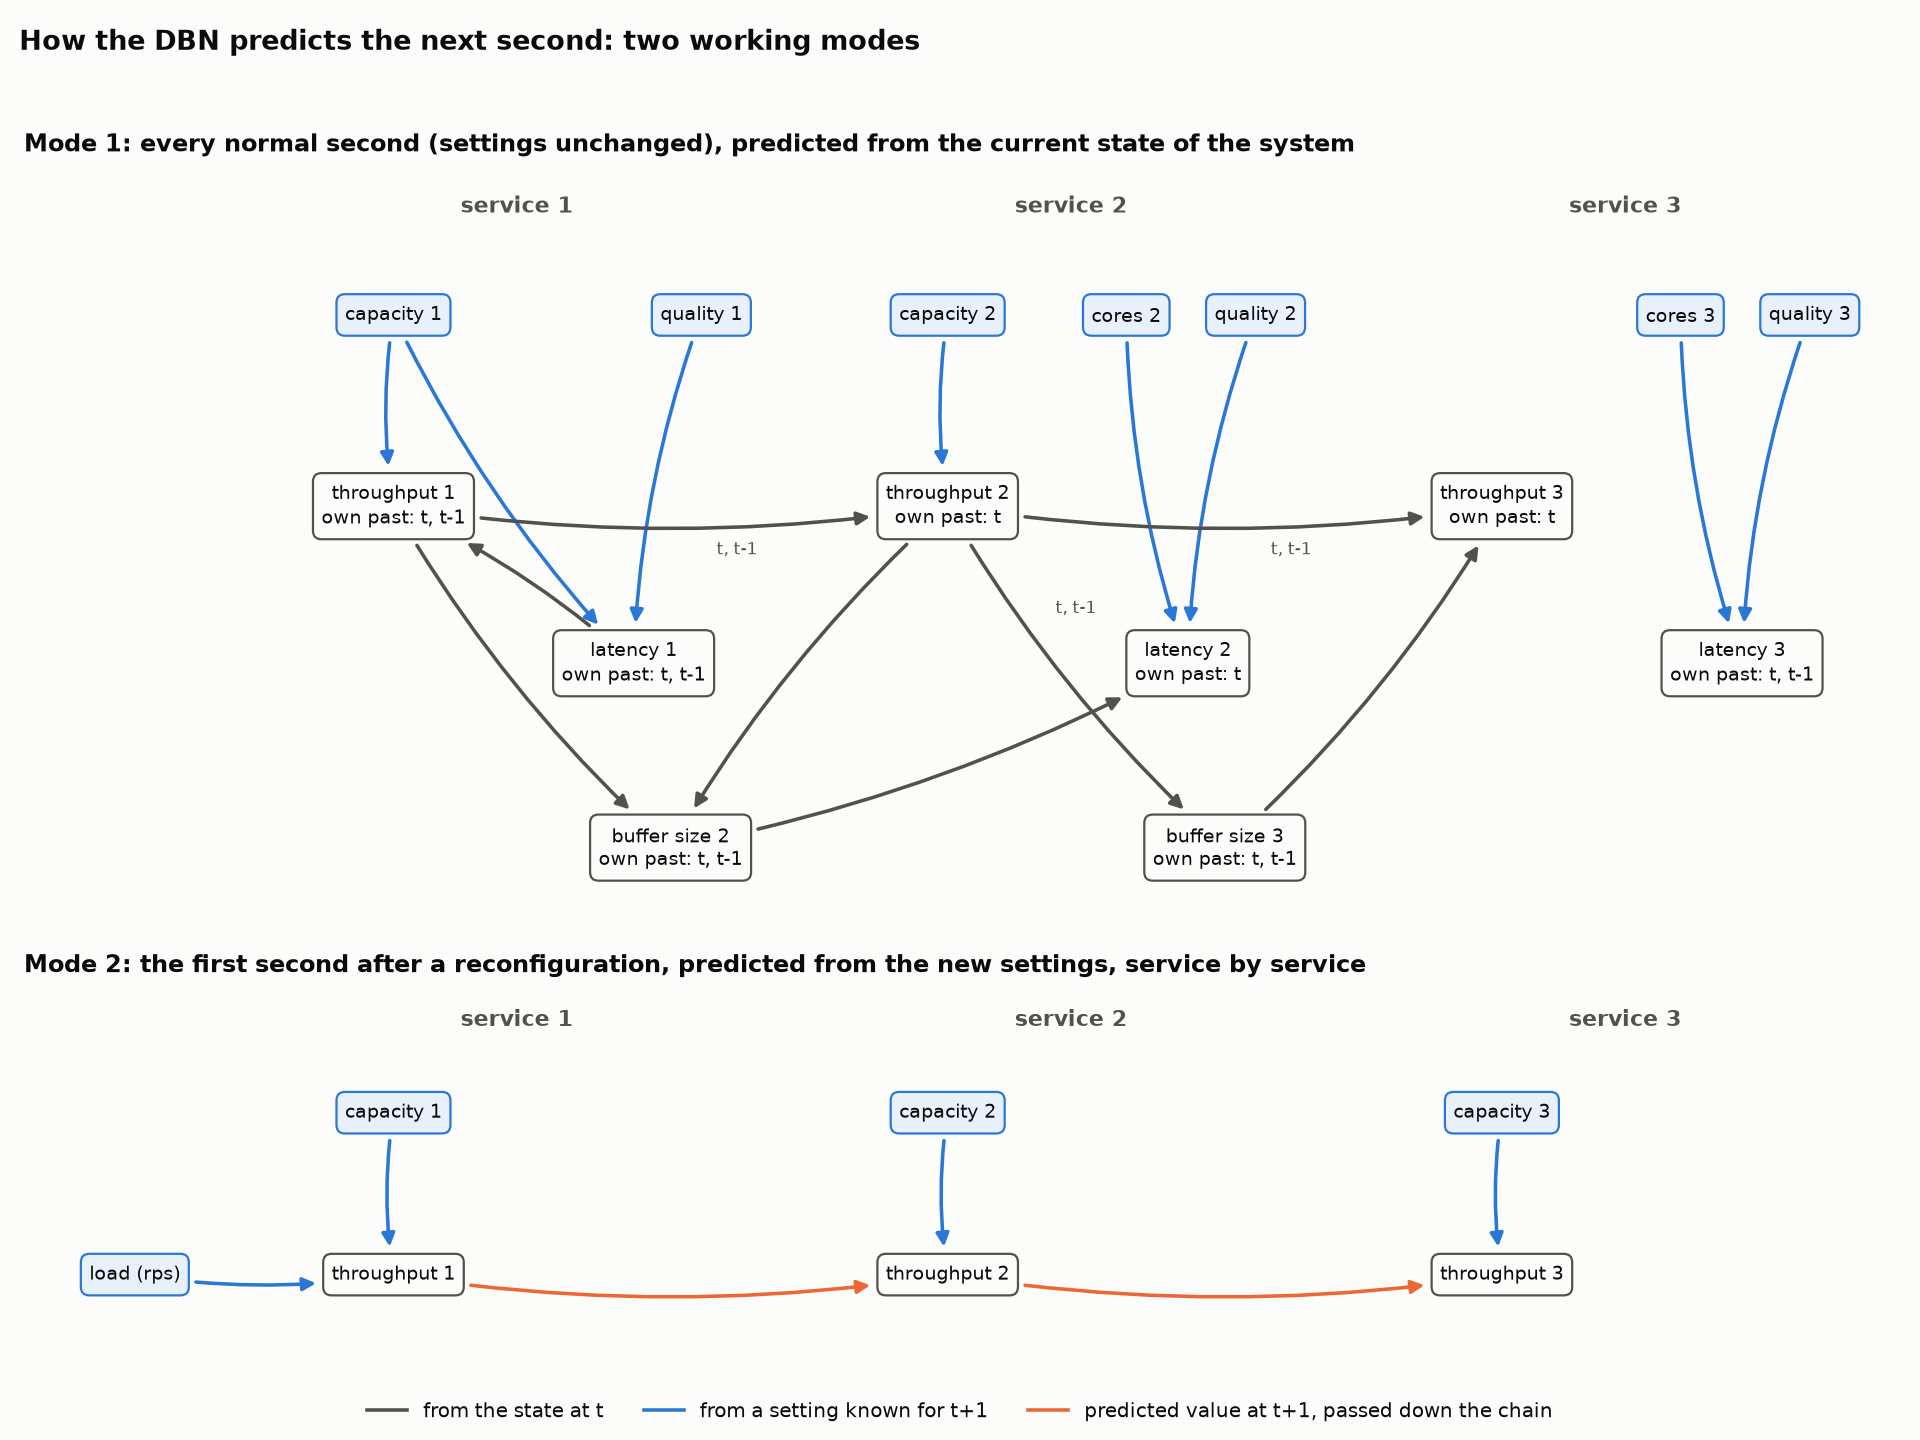
\includegraphics[width=\linewidth]{learned_structure.png}
  \caption{Structure of the final model, fitted on all runs of the three experiments.
  Mode~1: parents of every variable at an ordinary second; ``own past'' lists the variable's own values used as parents.
  Mode~2: at the first second after a reconfiguration, the throughputs are predicted from the new settings, service by service.
  The network topology was not given; candidate parents were only restricted to a service's own variables and the flow entering it.}
  \label{fig:structure}
\end{figure}

\subsection{Learning the model}
\label{sec:learning}

All steps below use the training runs of a fold only.

\paragraph{Discretisation.}
Each predicted variable is divided into 20 bins of equal width between its smallest and largest training value; the buffer sizes, which are zero most of the time, use 20 bins of equal frequency instead.
Throughputs, load and capacities measure the same quantity (requests per second) at different points of the chain and share one set of bin edges: the target's edges when the target is a throughput, otherwise 20 equal-width bins over their pooled training values.
Other continuous variables use 20 equal-frequency bins.
Variables with at most 20 distinct training values, such as cores and data quality, keep their values as categories.
Test values outside the training range fall into the outermost bins.

\paragraph{Capacity.}
For each service we add a derived exogenous variable, its capacity,
\begin{equation}
  \mathrm{capacity}_i = \mathrm{cores}_i \times r(q_i),
\end{equation}
where $r(q)$ is the number of requests one core processes per second at data-quality level $q$, the same function for all three services.
$r$ is learned from run means.
A service is saturated in a run when it emits less than 97\% of what it receives; in such runs its throughput equals its capacity, and $r(q)$ is the median of throughput$/$cores over saturated runs at that level (with at least three such runs).
In unsaturated runs throughput$/$cores is a lower bound of $r(q)$; where saturation is rare (low quality levels) this bound decides.
$r$ is then made non-increasing in $q$.
Inside cross-validation $r$ is learned from the first chunk of runs, which is training data in every fold; the final model learns it from all runs.

\paragraph{Candidate parents.}
The parents of a variable of service~$i$ are chosen among the variables of service~$i$ and the flow entering it (the load for service~1, throughput~$i-1$ otherwise): their values at $t$ and $t-1$, and, for settings and capacity, also at $t+1$.
The variable's own value at $t$ is always a parent.

\paragraph{Structure search.}
Parents are added by greedy forward selection judged on predictive performance.
The last 20\% of the training runs are held out; starting from the forced parent, each step fits the table with every remaining candidate added, keeps the candidate that lowers the held-out log-loss most, and stops when no candidate lowers it by more than $10^{-4}$ or when four parents are reached.
Because every candidate lies in an earlier slice or is exogenous, no choice can create a cycle.

\paragraph{Conditional probability tables.}
The table of $v$ given its parents is estimated by counting training pairs, with a Dirichlet prior of equivalent sample size $\alpha = 10$.
Instead of spreading the prior uniformly over the cells (BDeu), it is spread according to the autoregressive table $P_{\mathrm{AR}}(v_{t+1} \mid v_t)$, estimated on the same training data:
\begin{equation}
  P(v_{t+1} = k \mid \mathrm{pa} = j) = \frac{N_{jk} + \alpha\, P_{\mathrm{AR}}\bigl(k \mid v_t(j)\bigr)}{N_j + \alpha},
\end{equation}
where $N_{jk}$ counts training samples with parent configuration $j$ and next bin $k$, $N_j = \sum_k N_{jk}$, and $v_t(j)$ is the current bin of $v$ within configuration $j$.
A parent configuration never seen in training therefore predicts exactly as the autoregressive table, and a rare one is pulled towards it.

\paragraph{Mode 2: reconfiguration steps.}
At the first second after a reconfiguration the throughputs are predicted from the new settings and the current load, service by service.
Three tables $P(\mathrm{tp}_i \mid \mathrm{up}_i, \mathrm{capacity}_i)$, with $\mathrm{up}_1$ the load and $\mathrm{up}_i = \mathrm{tp}_{i-1}$ otherwise, are learned from all training samples with every value taken at the same second; they describe how a service responds to the flow it receives under a given capacity.
Their prior is centred on the bin of $\min(\mathrm{up}_i, \mathrm{capacity}_i)$, with 10\% of its mass on the neighbouring bins (a noisy-min prior).
The unobserved upstream throughputs at $t+1$ are summed out:
\begin{equation}
  P(\mathrm{tp}_3 \mid \mathrm{load}, c) = \sum_{\mathrm{tp}_1, \mathrm{tp}_2}
  P(\mathrm{tp}_1 \mid \mathrm{load}, c_1)\, P(\mathrm{tp}_2 \mid \mathrm{tp}_1, c_2)\, P(\mathrm{tp}_3 \mid \mathrm{tp}_2, c_3),
\end{equation}
where $c_i$ is the capacity of service~$i$ at $t+1$ and the load is the one observed at $t$.
Latencies and buffer sizes use mode~1 at every step.
Recorded seconds after a reconfiguration begin at least 30\,s after the change (Section~\ref{sec:data}), so mode~2 predicts the state the chain has settled into under the new settings, not the transient that follows the change.
Giving the chain the load of the predicted second instead, which is known in these experiments from the workload schedule, changes accuracy at reconfigurations from 0.643 to 0.652 and overall accuracy by less than 0.01 percentage points.

\paragraph{Numeric forecasts.}
To report errors in requests per second, the model is also read out as a number.
For each parent configuration we take the median change $v_{t+1} - v_t$ observed in training (at least five samples; otherwise the median change for the current bin of $v$) and add it to the observed $v_t$.
At reconfiguration steps the expected bin value of the mode-2 distribution is used.

\subsection{Evaluation}
\label{sec:evaluation}

\paragraph{Cross-validation.}
Each experiment is evaluated separately with expanding-window cross-validation over whole runs.
The 560 runs, in the order they were executed, are cut into six consecutive chunks at run boundaries; fold $k$ ($k = 1, \dots, 5$) trains on chunks 1 to $k$ and tests on chunk $k+1$.
A run is never split between training and test, and a sample belongs to the run of its predicted second.
Every model and baseline is scored on exactly the same test samples: 467 test runs per experiment, 1{,}401 over the three.

\paragraph{Baselines.}
\begin{itemize}
  \item \emph{Persistence}: the next bin equals the current bin.
  \item \emph{Autoregressive table (AR)}: $P(v_{t+1} \mid v_t)$ on the same bins, BDeu prior with $\alpha = 10$. It is the DBN restricted to its forced parent and the reference for every comparison.
  \item \emph{Gradient boosting}: a histogram gradient-boosting regressor with fixed hyperparameters (absolute-error loss, 300 iterations, learning rate 0.05) predicting the change $v_{t+1} - v_t$.
  \item \emph{TabPFN v3.5}~\cite{tabpfn}: a tabular foundation model predicting the change $v_{t+1} - v_t$, conditioned on 10{,}000 training samples drawn at random from the fold's training runs (its context limit).
\end{itemize}
Gradient boosting and TabPFN receive exactly the columns the DBN can read (Table~\ref{tab:inputs}): its candidate parents and the inputs of the reconfiguration chain.
The three learned models therefore have the same information; they differ only in how they use it.
All models are scored on the same 2{,}000 test samples per fold.

\begin{table}[t]
  \centering
  \caption{Inputs of each model for throughput~3. No model receives the load of the predicted second.}
  \label{tab:inputs}
  \begin{tabular}{p{0.24\linewidth}p{0.68\linewidth}}
    \toprule
    Model & Inputs \\
    \midrule
    Persistence & throughput~3 at $t$ \\
    AR table & bin of throughput~3 at $t$ \\
    DBN, gradient boosting, TabPFN &
      at $t$ and $t-1$: throughput~3, throughput~2, latency~3, buffer size~3, cores~3, data quality~3, capacity~3;
      at $t$: the load;
      at $t+1$: cores~3, data quality~3, capacity of services 1, 2 and 3 \\
    \bottomrule
  \end{tabular}
\end{table}

The DBN uses these columns in two parts: its tables at ordinary seconds choose their parents among the columns of service~3 and throughput~2, and the chain at reconfigurations reads the load and the three capacities.

\paragraph{Metrics.}
\emph{Accuracy} is the share of test samples whose most probable bin is the observed bin.
\emph{Log-loss} is the mean of $-\log P(\text{observed bin})$, with probabilities floored at $10^{-12}$.
We also report macro F1 over bins and the \emph{mean absolute error} (MAE) of the numeric forecast in the variable's units.
\emph{Accuracy at change} is the accuracy on the samples whose bin changes between $t$ and $t+1$; persistence scores zero there by construction, so it isolates what a model predicts beyond ``no change''.
\emph{Accuracy at reconfiguration} is the accuracy on the first second after a reconfiguration.

\paragraph{Statistical comparison.}
Two configurations, or a configuration and the AR table, are compared on the test runs they share by a paired bootstrap with 10{,}000 resamples.
The three experiments visit the same configuration schedule, so run $k$ of each experiment is the same experimental condition under a different load; the unit of resampling is therefore the position in the schedule (467 positions in the test folds), with the runs of the three experiments at that position drawn together.
We report the difference in each metric with its 95\% percentile interval and a two-sided bootstrap $p$-value, Holm-corrected for the number of configurations compared within a study.

\paragraph{Ablation design.}
The modelling options were studied on throughput~3 at 1\,s with 20 bins, starting from a reference configuration and changing one option at a time (60 configurations): number of bins and discretisation method, history length of the target and of the other variables, velocity features, candidate pool, exogenous inputs, structure-search method (cross-validated forward selection; hill climbing with BIC, AIC or BDeu; conditional mutual information; Lasso ranking; DYNOTEARS~\cite{dynotears}; a fixed expert parent set), table prior and its sample size, maximum number of parents, and the treatment of reconfiguration steps.
Options that interact were crossed in a factorial design (128 configurations: bins $\times$ history length $\times$ search method $\times$ maximum parents $\times$ relative inputs).
Further studies varied the resolution (1, 5, 10, 30\,s) and number of bins jointly, the prediction horizon, the cross-validation scheme (expanding vs.\ blocked), the capacity variable and the reconfiguration chain.
The options whose effect was positive and significant were combined into the recommended configuration (Section~\ref{sec:learning}), which was then evaluated on all eight variables with 20 and 50 bins, and on throughput~3 at 30\,s with 4, 10 and 20 bins.

\paragraph{Held-out-pattern check.}
Because the options were chosen on the same three experiments the configuration is evaluated on, the choice was repeated without each experiment in turn.
For each held-out pattern, the options (history length of the target and of the other variables, velocity, candidate pool, search method, prior, maximum parents, reconfiguration treatment) were chosen by coordinate ascent on the pooled cross-validated accuracy of the other two patterns, and the chosen configuration was then scored on the held-out pattern.
In all three rounds the selection reached the recommended configuration up to two options without measurable effect (three instead of two lags of the other variables; at most six instead of four parents).
On the held-out pattern it scored 0.929, 0.922 and 0.919 for periodic, once-in-a-lifetime and unpredictable load, against 0.926, 0.924 and 0.916 for the recommended configuration and 0.887, 0.872 and 0.866 for the AR table (gains over AR $+0.042$ [0.035, 0.050], $+0.050$ [0.041, 0.059], $+0.053$ [0.044, 0.064]; run-level bootstrap within the pattern).
The selection therefore does not inflate the reported results.

\paragraph{Final model.}
For inspection and use, the recommended configuration is fitted once on all runs of the three experiments (1{,}680 runs); its parent sets are those shown in Figure~\ref{fig:structure}.
Its accuracy on the data it was fitted on is not reported as a result; all reported scores are cross-validated.

\paragraph{Further analyses.}
\begin{itemize}
  \item \emph{Several seconds ahead}: the one-step tables of the five flow variables (throughputs and buffer sizes) are unrolled with 100 particles for 1 to 30\,s and compared with tables trained directly for each horizon.
  \item \emph{Unseen configurations}: at 30\,s resolution, the throughputs are predicted from the load and the settings alone, in folds where most test core allocations never occur in training. Every learned comparison model, TabPFN included, is run both on the raw settings (cores, data quality) and on the capacities, so that the comparison separates the model from the input.
  \item \emph{Detecting reconfigurations}: the surprise $-\log P(\text{observed})$ of the network's nodes, summed over a node set, is used as an alarm score; its threshold for 1\% false alarms is set on one half of the test runs and evaluated on the other half (1\,s resolution).
\end{itemize}

\subsection{Implementation and reproducibility}

The pipeline is implemented in Python~3.12 with NumPy, pandas, SciPy and scikit-learn; tables, structure search and inference are implemented directly as counting over discretised columns and checked against pgmpy~0.1.26 (identical probabilities and BIC scores for the same parent set).
All random choices use fixed seeds, so the analysis is deterministic: rerunning it on the same data and code reproduces every number exactly.
Code, result tables and the final model are available at \url{https://github.com/NefeliRouska/dbn_model_construction} \tocheck{commit or tag to cite}; the raw monitoring data (about 14\,GB) are available on request \tocheck{where they will be archived}.

% ---------------------------------------------------------------------------
% Limitations: move to the Discussion section of the paper.
% - The three experiments share one configuration schedule; they are three load patterns
%   over the same 560 conditions, not independent samples of configurations.
% - The recommended configuration was selected on the same experiments it is evaluated on;
%   the held-out-pattern check shows that choosing without a pattern gives the same accuracy on it.
% - The load is the setpoint seen by service 1, not a measured arrival rate. The settings for
%   the next second are assumed known (a controller decides them); the load is not.
% - Recorded data start >= 30 s after each reconfiguration: the model predicts the settled
%   state, not the transient after a change.
% - Gradient boosting uses fixed hyperparameters; TabPFN is limited to a 10,000-sample context.
% - One testbed with three services in a fixed chain.
% ---------------------------------------------------------------------------

\begin{thebibliography}{9}
  \bibitem{sedlak_workbench} \tocheck{Sedlak et al., elastic-workbench: full reference.}
  \bibitem{tabpfn} \tocheck{TabPFN v3.5 (Prior Labs): full reference.}
  \bibitem{dynotears} R.~Pamfil et al., ``DYNOTEARS: Structure learning from time-series data,'' in \emph{Proc.\ AISTATS}, 2020.
\end{thebibliography}

\end{document}
